\documentclass[10pt,a4paper]{article}
\usepackage[utf8]{inputenc}
\usepackage[english]{babel}
\usepackage{amsmath}
\usepackage{amsfonts}
\usepackage{amssymb}
\usepackage{graphicx}
\usepackage{natbib}
\usepackage{fullpage}
\author{Pierre Gloaguen, Marie-Pierre \'Etienne and Sylvain Le Corff}
\title{A continuous time movement model linking displacement to utilization distribution}

%%%%% Commands
\newcommand{\Ar}{\mathcal{A}}
\newcommand{\PR}{\mathbb{P}}
\newcommand{\rmd}{\text{d}}
\newcommand{\ud}{\boldsymbol{\pi}}
\begin{document}
\maketitle
\abstract{This paper introduces a new continuous time and continuous space movement model, to describe animal's movement as the consequence of its environment quality and availability. The model depicts the position process as a diffusion process, solution to a  Stochastic Differential Equation (SDE), with an explicit stationary distribution. This stationary distribution might be understood as the the utilization distribution of the animal. The explicit mechanistic formulation through a stochastic differential equation allows the estimation of the utilization distribution using classical estimation methods for diffusion processes. This estimation allows the ecologist to test for the effect of any habitat preference on the utilization distribution, as well as to infer metrics of exploration tendency for a given individual.}

\section{Introduction}
In movement ecology, a challenging question is to relate individuals movement to habitat preferences. As a proxy of an animal habitat preferences, ecologists often rely on the utilization distribution of the individual, that is the probability density function $\ud$ such that, for an area $\Ar$ of the space, if $X \in \mathbb{R}^d$ denotes the position of the animal of interest:
$$\PR(X \in \Ar) = \int_{\Ar} \ud(z) \rmd z\,.$$

Environmental impact assessment and conservation measure require to predict the effect of a change on spatial environmental variables and therefore require knowledge on the link between environment variables and utilization distribution function. This link might be studied by incorporating  $K$ spatial covariates function $c_1, \dots, c_K$, in the utilization distribution function $\ud$  and their effects summed up in a parameter $\theta$ such that: 
\begin{equation}
\label{eq:ParUD}
\ud(z) = \ud (\theta, c_1(z), \dots, c_K(z))\,.
\end{equation}
In movement ecology, it is widely admitted that animal movement is related to the utilization distribution, as movement eventually leads to an overall space use. Indeed, movement data is often used to infer utilization distribution, either with kernel density methods \citep{worton1989kernel, fleming2015rigorous} or Brownian bridges methods \citep{horne2007analyzing}. However, there exist few works to mechanistically link movement to the utilization distribution in a movement model. This would require to have a realistic movement model whose stationary distribution is the targeted utilization distribution.
Recently  \citet{michelot2017linking} proposed a step selection movement model, explicitly based on the utilization distribution. This approach describes the individual's movement as a Markov chain whose stationary distribution is the utilization distribution. Markov Chain Monte Carlo (MCMC) algorithms may then be proposed to sample from the target stationary distribution. In this case, the authors used a local Gibbs sampler.

On the other hand, mechanistic movement model have been proposed where the individual's movement is a direct consequence of the environment \citep{brillinger2010handbook}. In this approach, the individual's position is supposed to follow the gradient of a potential surface whose value reflects the potential interest for the animal \citep{preisler2013analyzing}. These Markovian approaches offer a wide variety of flexible models to describe movement, but there relation to utilization distribution is unclear in the existing examples as the diffusion process are not stationary \citep{gloaguen2017stochastic}  or lead to unrealistically simple utilization distribution (by example a uniform distribution for a Brownian motion movement model or a normal distribution for an Ornstein Uhlenbeck based movement model).

In this work, we propose a mechanistic movement model gathering the ideas of \citet{brillinger2010handbook} (the movement is a diffusion process whose drift is the gradient of a potential surface) and of \citet{michelot2017linking} (the stationnary distribution of the animal's position is its  utilization distribution). The movement model is based on the Langevin diffusion, known as the base of a particular MCMC algorithm \citep{roberts1998optimal}.

As this model belongs to the class of potential based models, inference can be performed from movement data using different estimation methods for stochastic differential equations (SDEs), such as pseudo likelihood methods which are easy to implement \citep{gloaguen2017stochastic}.

In section \ref{sec:model}, we formulate the proposed movement model. In section \ref{sec:inference}, we briefly recall the inference method used in this work and present some results on simulated data.
\section{Langevin movement model}
\label{sec:model}

We here consider an individual moving in its environment in $\mathbb{R}^d$, $d=2$ mostly but might be equal to $3$ in marine ecology, where the depth is of importance. We suppose that the individual has a utilization distribution $\ud:~\mathbb{R}^d  \mapsto  \mathbb{R}$, potentially defined with a central parameter and  the effect of some covariates, as in equation \eqref{eq:ParUD}. We assume moreover that $\ud(z)$ is strictly positive on $\mathbb{R}^d$, and that $\log \ud(z)$ is smooth.

We suppose that the continuous time position process $(X_t)_{t\geq 0}$ is the solution to the following stochastic differential equation:
\begin{equation}
\label{eq:Langevin}
\rmd X_t = \frac{1}{2}\nabla_z \log \ud(X_t) \rmd t + \rmd W_t,~~X_0 = x_0
\end{equation}
where $W_t$ is a standard $d$-dimensional Brownian motion and $x_0$ is the initial position of the animal. Under some mild technical conditions (that can be found in \citet{dalalyan2017theoretical}), the SDE  \eqref{eq:Langevin} has a unique solution. This solution is a continuous time Markov process whose stationary distribution is $\ud$ \citep{roberts1996exponential}. 

\subsection{Example}
We here consider an example to show how the equation \eqref{eq:Langevin} can be used to simulate a trajectory from an individual having a known utilization distribution. We consider the following utilization distribution:
\begin{equation}
\label{eq:ExUD}
\ud(z) \propto \exp\left( \alpha\parallel z - \mu\parallel^2 + \beta_1 c_1(z) + \beta_2 c_2(z) \right)\,.
\end{equation}
where:
\begin{itemize}
\item $c_1(z)$ and $c_2(z)$ are smooth covariates whose gradient are assumed to be known for every $z$. A simple case, would be a linear effect of the covariates, but more complex effect can be modelled with some smooth transformation of the covariates. The example of covariates presented here are shown on Figure \ref{fig:Covariates} ;
\item $\beta_1$ and $\beta_2$ are parameters indicating whether the following covariate has an attractive (positive sign) or repulsive (negative sign) effect on the individual's movement. For this example we set $\beta_1 = -1$ and $\beta_2 = 0.5$ ;
\item $\mu$ is a home parameter, defining a point from which the animal tends to stay close. This point might reflect a nest or a burrow, or only the abstract center of a zone the animal does not quit for a long time. It is here fix to the center of the map (the 0 point) ;
\item $\alpha$ is a concentration parameter around the point $\mu$. The higher alpha is, the closer the animal tends to stay to $\mu$.
In the example, it is fixed to 0.05.
\end{itemize}
The resulting distribution given by \eqref{eq:ExUD} is shown in Figure \ref{fig:ResultUD}.

\paragraph{Simulations according to the Langevin model} The solution to equation \eqref{eq:Langevin} is a Markov process. However, for most cases, even with known parameters, there is no procedure to get sample exactly a solution to \eqref{eq:Langevin}. Indeed, for a vast majority of diffusion processes, the probablity density function of $X_{t}$ given  $X_0$ has no explicit form, thus there is no straightforward exact sampling algorithm.



However, some simple approximation schemes exist, such as the Euler scheme. This scheme can be used to sample approximations of the Langevin diffusion in the following way: from a starting point $x_0$, and given an approximation time step $h$, sample $x_{t+h}$ as:
\begin{equation}
\label{eq:EulerScheme}
x_{t+h} = x_t + \nabla \log \ud(x_t)\times h +\varepsilon_t,~\varepsilon \sim \mathcal{N}_d\left(0, h\times I_d\right)
\end{equation} 
This approximation is valid  when $h$ goes to 0. Indeed, it is strongly recommended to choose a small value for $h$ so that the approximation remains valid \citep{roberts1996exponential}.
An example of an approximated trajectory starting from $\mu$ obtained using the Euler scheme is shown in Figure \ref{fig:ExampleTrajectory}. More sophisticated approximate schemes might be explored (\citealp{gloaguen2017stochastic}) with no restriction on the choice of the utlization distribution, while the exact sampling scheme (\citealp{beskos2006exact}) imposes resctritive assumptions on $\mathbf{\pi}$.

Despite the bimodal utilization distribution, the trajectory tends to explore the overall area and switches frequently from one mode to the other. Figure~\ref{fig:GradientNorm} shows the norm of $\nabla \log \ud(z)$, i.e. the drift of the SDE.
\begin{figure}
\centering
\begin{tabular}{cc}
$c_1(z)$ & $c_2(z)$\\
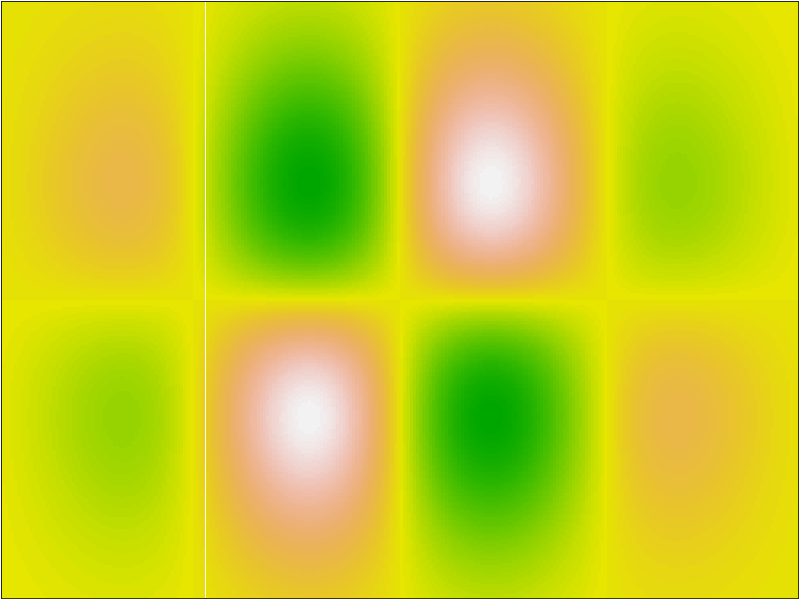
\includegraphics[width = 0.48\textwidth]{figures/Covariate1}&
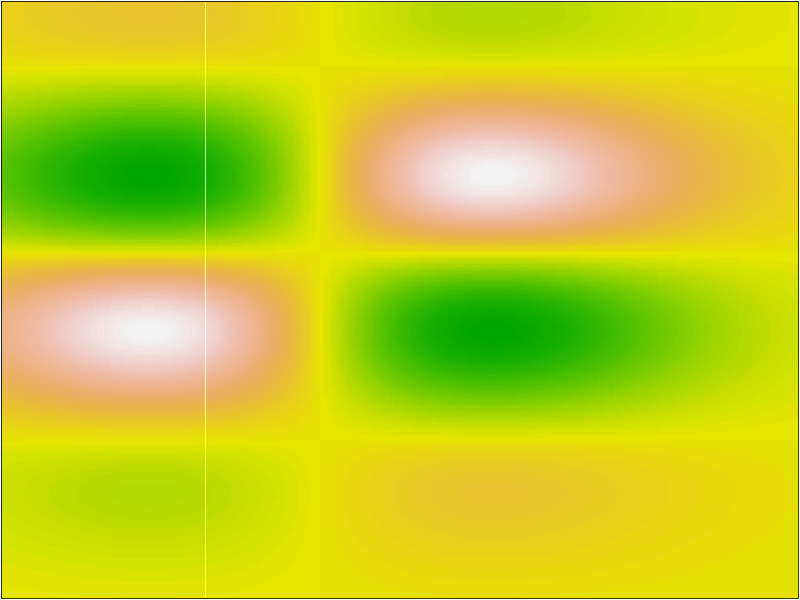
\includegraphics[width = 0.48\textwidth]{figures/Covariate2}
\end{tabular}
\caption{\label{fig:Covariates} Two covariates patches for our example. Higher values are in white, lower values are in green. The covariate $c_1$ is supposed to be repulsive, the covariate $c_2$ is supposed to be attractive.}
\end{figure}
\begin{figure}
\centering
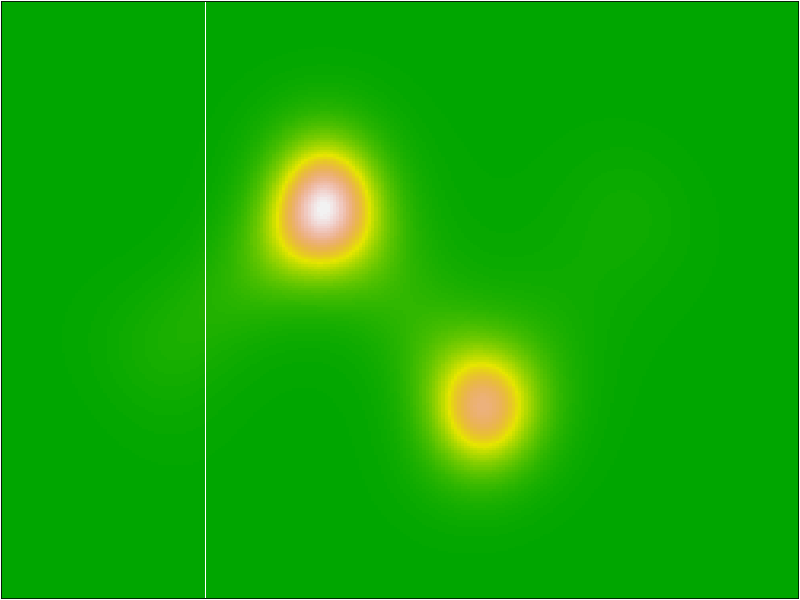
\includegraphics[width = 0.48\textwidth]{figures/ResultingUD}
\caption{\label{fig:ResultUD} Utilization distribution for our example. This distribution is the result of equation \eqref{eq:ExUD} with parameters given in the text, and covariates of Figure \ref{fig:Covariates}.}
\end{figure}
\begin{figure}
\centering
\begin{tabular}{ccc}
$\ud(z)$&$c_1(z)$&$c_2(z)$\\
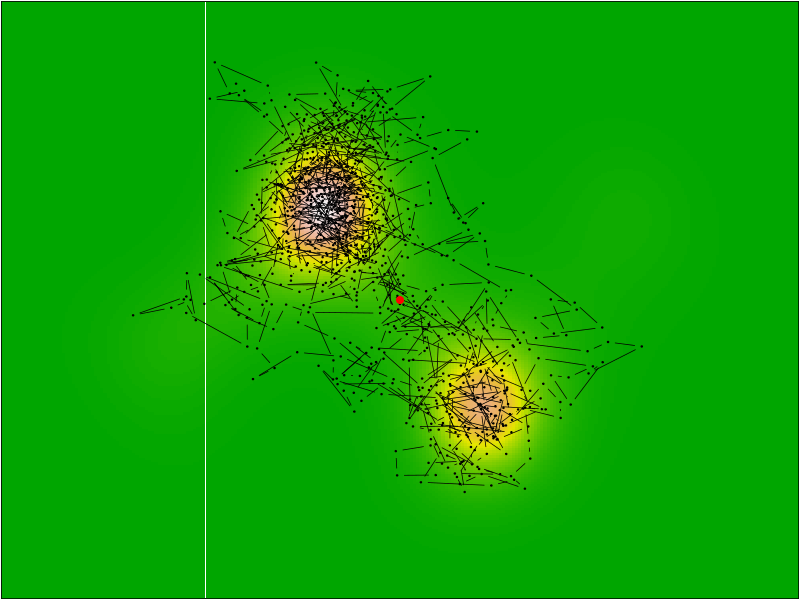
\includegraphics[width = 0.32\textwidth]{figures/TrajPlusUD}&
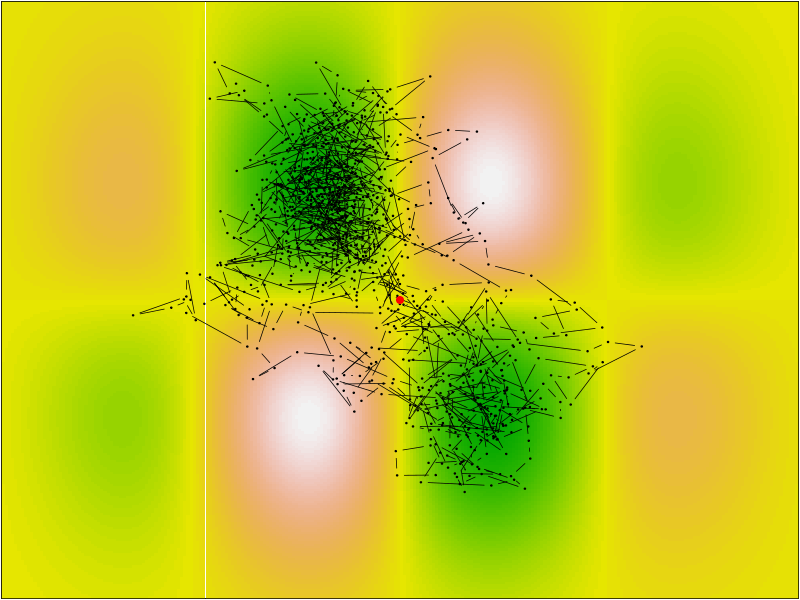
\includegraphics[width = 0.32\textwidth]{figures/TrajPlusC1}&
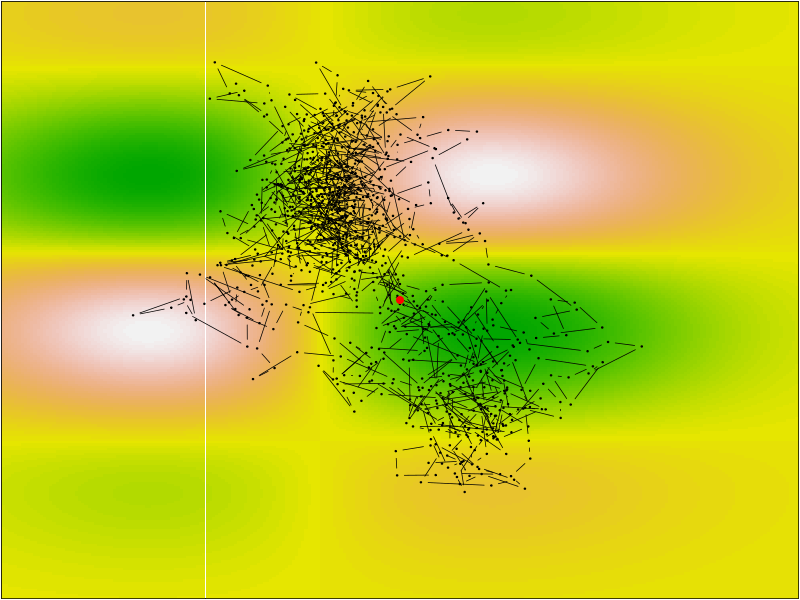
\includegraphics[width = 0.32\textwidth]{figures/TrajPlusC2}
\end{tabular}
\caption{\label{fig:ExampleTrajectory} Example of a sampled trajectory using the Euler scheme $n = 1000$. The trajectory is plotted against the utilization distribution and the two covariates fields.}
\end{figure}
\begin{figure}
\centering
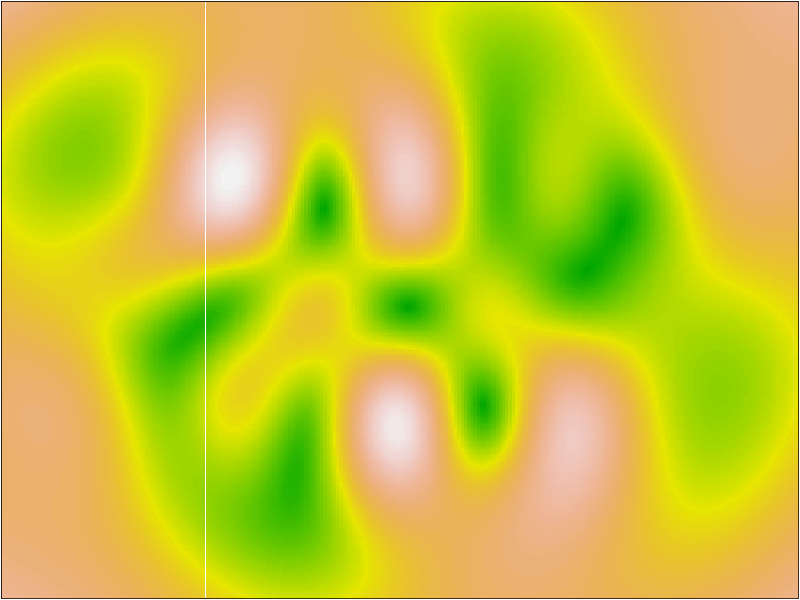
\includegraphics[width = 0.48\textwidth]{figures/GradientNorm}
\caption{\label{fig:GradientNorm} Gradient of $\nabla \log \ud(z)$. The greener, the lower, the whiter, the greater.}
\end{figure}
\section{Inference}
\label{sec:inference}
An important question in ecology is the inference of habitat preferences that shape the utilization distribution. In this context, given a parametric form for $\ud(z)$ as in \eqref{eq:ParUD} or \eqref{eq:ExUD}, the objective is to infer $\theta$ from movement data. We suppose, for an individual, that data consists in a set of $n$ points $\mathbf{x} :=(x_1, \dots, x_n)$ sampled at times $t_1< t_2<\dots < t_n$. We suppose that this sample is a realisation of the process solution to \eqref{eq:Langevin}. This solution is a Markov process, therefore, the  likelihood is given by:
\begin{equation}
\label{eq:LangLikelihood}
L(\theta\vert \mathbf{x}) = \sum_{i = 1}^{n - 1} p(x_{i+1}\vert x_i, \theta, \Delta_i)\,,
\end{equation}
where $\Delta_i = t_{i+1} - t_i$, and  $p(\cdot\vert x_i, \theta, \Delta_i)$ is the p.d.f. of the law of $X_{t_i + \Delta_i}$ given that the process is at $x_i$ at time $t_i$ when the parameter is $\theta$. 

However, as said above, this p.d.f. is impossible to compute in general. Different estimation methods exist to circumvent this problem \citep{gloaguen2017stochastic}. Here, as a proof of concept, we choose to perform the estimation using the Euler-Maruyama approximation. 

This method consists in replacing $p(\cdot\vert x_i, \theta, \Delta_i)$ in equation \eqref{eq:LangLikelihood} by the p.d.f. of a Gaussian distribution with mean $x_i + \nabla \log \ud(z, \theta)\times \Delta_i$ and variance $\Delta_i \times I_d$, as suggested by \eqref{eq:EulerScheme}\footnote{This method is known to perform poorly when the sampling time step becomes too large, and could be replaced by other pseudo likelihood methods, such as the Ozaki method}.
\subsection{Inference on simulated data}
For any utilization distribution, the pseudo likelihood induced by the Euler approximation can be maximized using gradient ascent algorithm. 

An example for the model considered here is given for a subsample of the simulations in Figure \ref{fig:ExampleTrajectory}, with $n = 500$ and $\Delta$ = 1. Parameters $\alpha$, $\beta_1$ and $\beta_2$ are estimated with 10 random starting points. The overall procedure takes less than one second. Results are shown in Figure \ref{fig:ParamsEstimation}. The algorithm converges after 3 iterations. 

To assess whether, at this time step, the estimation is biased, the procedure is repeated for 100 similarly simulated trajectories and the associated boxplots are given in Figure \ref{fig:BoxplotParams}. This shows an underestimation of parameter norms. This is expected at this time step, and might be accentuated by the Euler procedure.

\section{Discussion}

This preliminary work proposes a movement model linking movement to utilization distribution and habitat preferences. In this model, the path of an animal is considered as the solution to a Langevin diffusion. From this point of views, it presents strong analogies with the sampling scheme  based on MCMC methods proposed by \cite{michelot2017linking}. As the model belongs to a known class of potential based diffusion processes, classical pseudo likelihood approaches can be used to estimate utilization distribution parameters from movement data. 

This allows to test the influence of habitat covariates, as well as remoteness from a given point. On the example presented here (similar to the one of \citealp{michelot2017linking}), parameter estimation is fast and explicit.

\begin{figure}
\centering
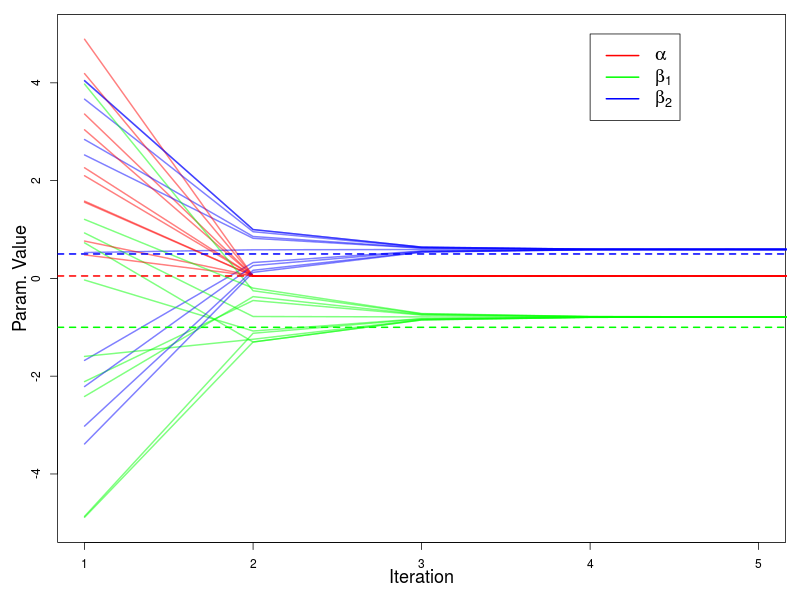
\includegraphics[width = 0.48\textwidth]{figures/ParamEstimation}
\caption{\label{fig:ParamsEstimation} Estimations of $\alpha$, $\beta_1$ and $\beta_2$ using a subsample of the trajectory of Figure \ref{fig:ExampleTrajectory}, using 10 starting points for our estimation algorithm. True values for each parameter is the dotted line. The estimation converges after 3 iterations.}
\end{figure}
\begin{figure}
\centering
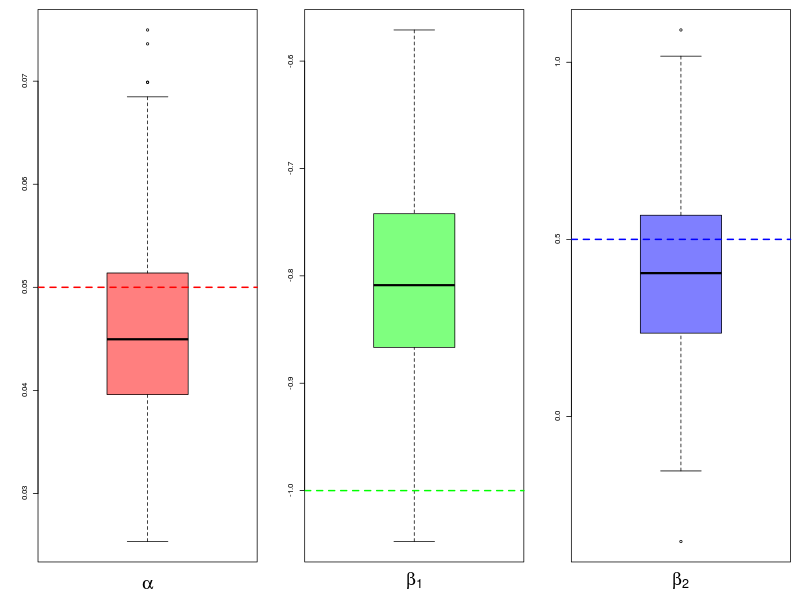
\includegraphics[width = 0.48\textwidth]{figures/BoxplotParams}
\caption{\label{fig:BoxplotParams} Boxplot of 300 independant estimates obtained on 300 independant trajectories with $\Delta = 1$. The bias is due to the large time step. It could also be due to the Euler approximation.}
\end{figure}
\bibliographystyle{apa}
\bibliography{Biblio}
\end{document}